Determining the water density in the beam at the ion trap is more difficult than in the CBGB and stem region. During normal operation of the CBGB, neither the RGA, nor the ion gauge in the trap chamber, which are off the beam axis and in a nipple, are able to detect a change in the background water pressure. With the characterization of the \ce{Be+ + H2O} reaction pathways, we were able to validate both experimentally and theoretically, the rate constant and that it follows the ADO model (Section \ref{sec: Be+H2O}). By extending the rate of the \ce{Be+ + H2O} reaction complex to whatever reaction temperature is achieved by the CBGB entrained water (equation \ref{eq: k Be+H2O(T)}), we may monitor either the fluorescence decay, or the time evolution of the time of flight mass spectrometer (TOF-MS discussed in Section \ref{sec: TOF}) peaks to extrapolate a \ce{H2O} density. Furthermore, if the peaks of the reaction products of \ce{Be+} and other trapped ions do not overlap, we may determine the beam density for each set of time resolved TOF traces individually.

When probing the reactions of \ce{C+ + H2O} discussed in Section \ref{sec: [HCO]}, the reaction reaction products of \ce{[HCO]+} and \ce{H3O+} have $m/z=$29 and 19, respectively, without conflict with \ce{Be+} or \ce{BeOH+} ($m/z=26$), the main reaction product of \ce{Be+ + H2O} as seen in Figure \ref{fig: Be+CO+H2O+CO all traces}.

\begin{figure}[H]
	\centering
	\makebox[\textwidth][c]{
	\begin{tabular}{cc}
		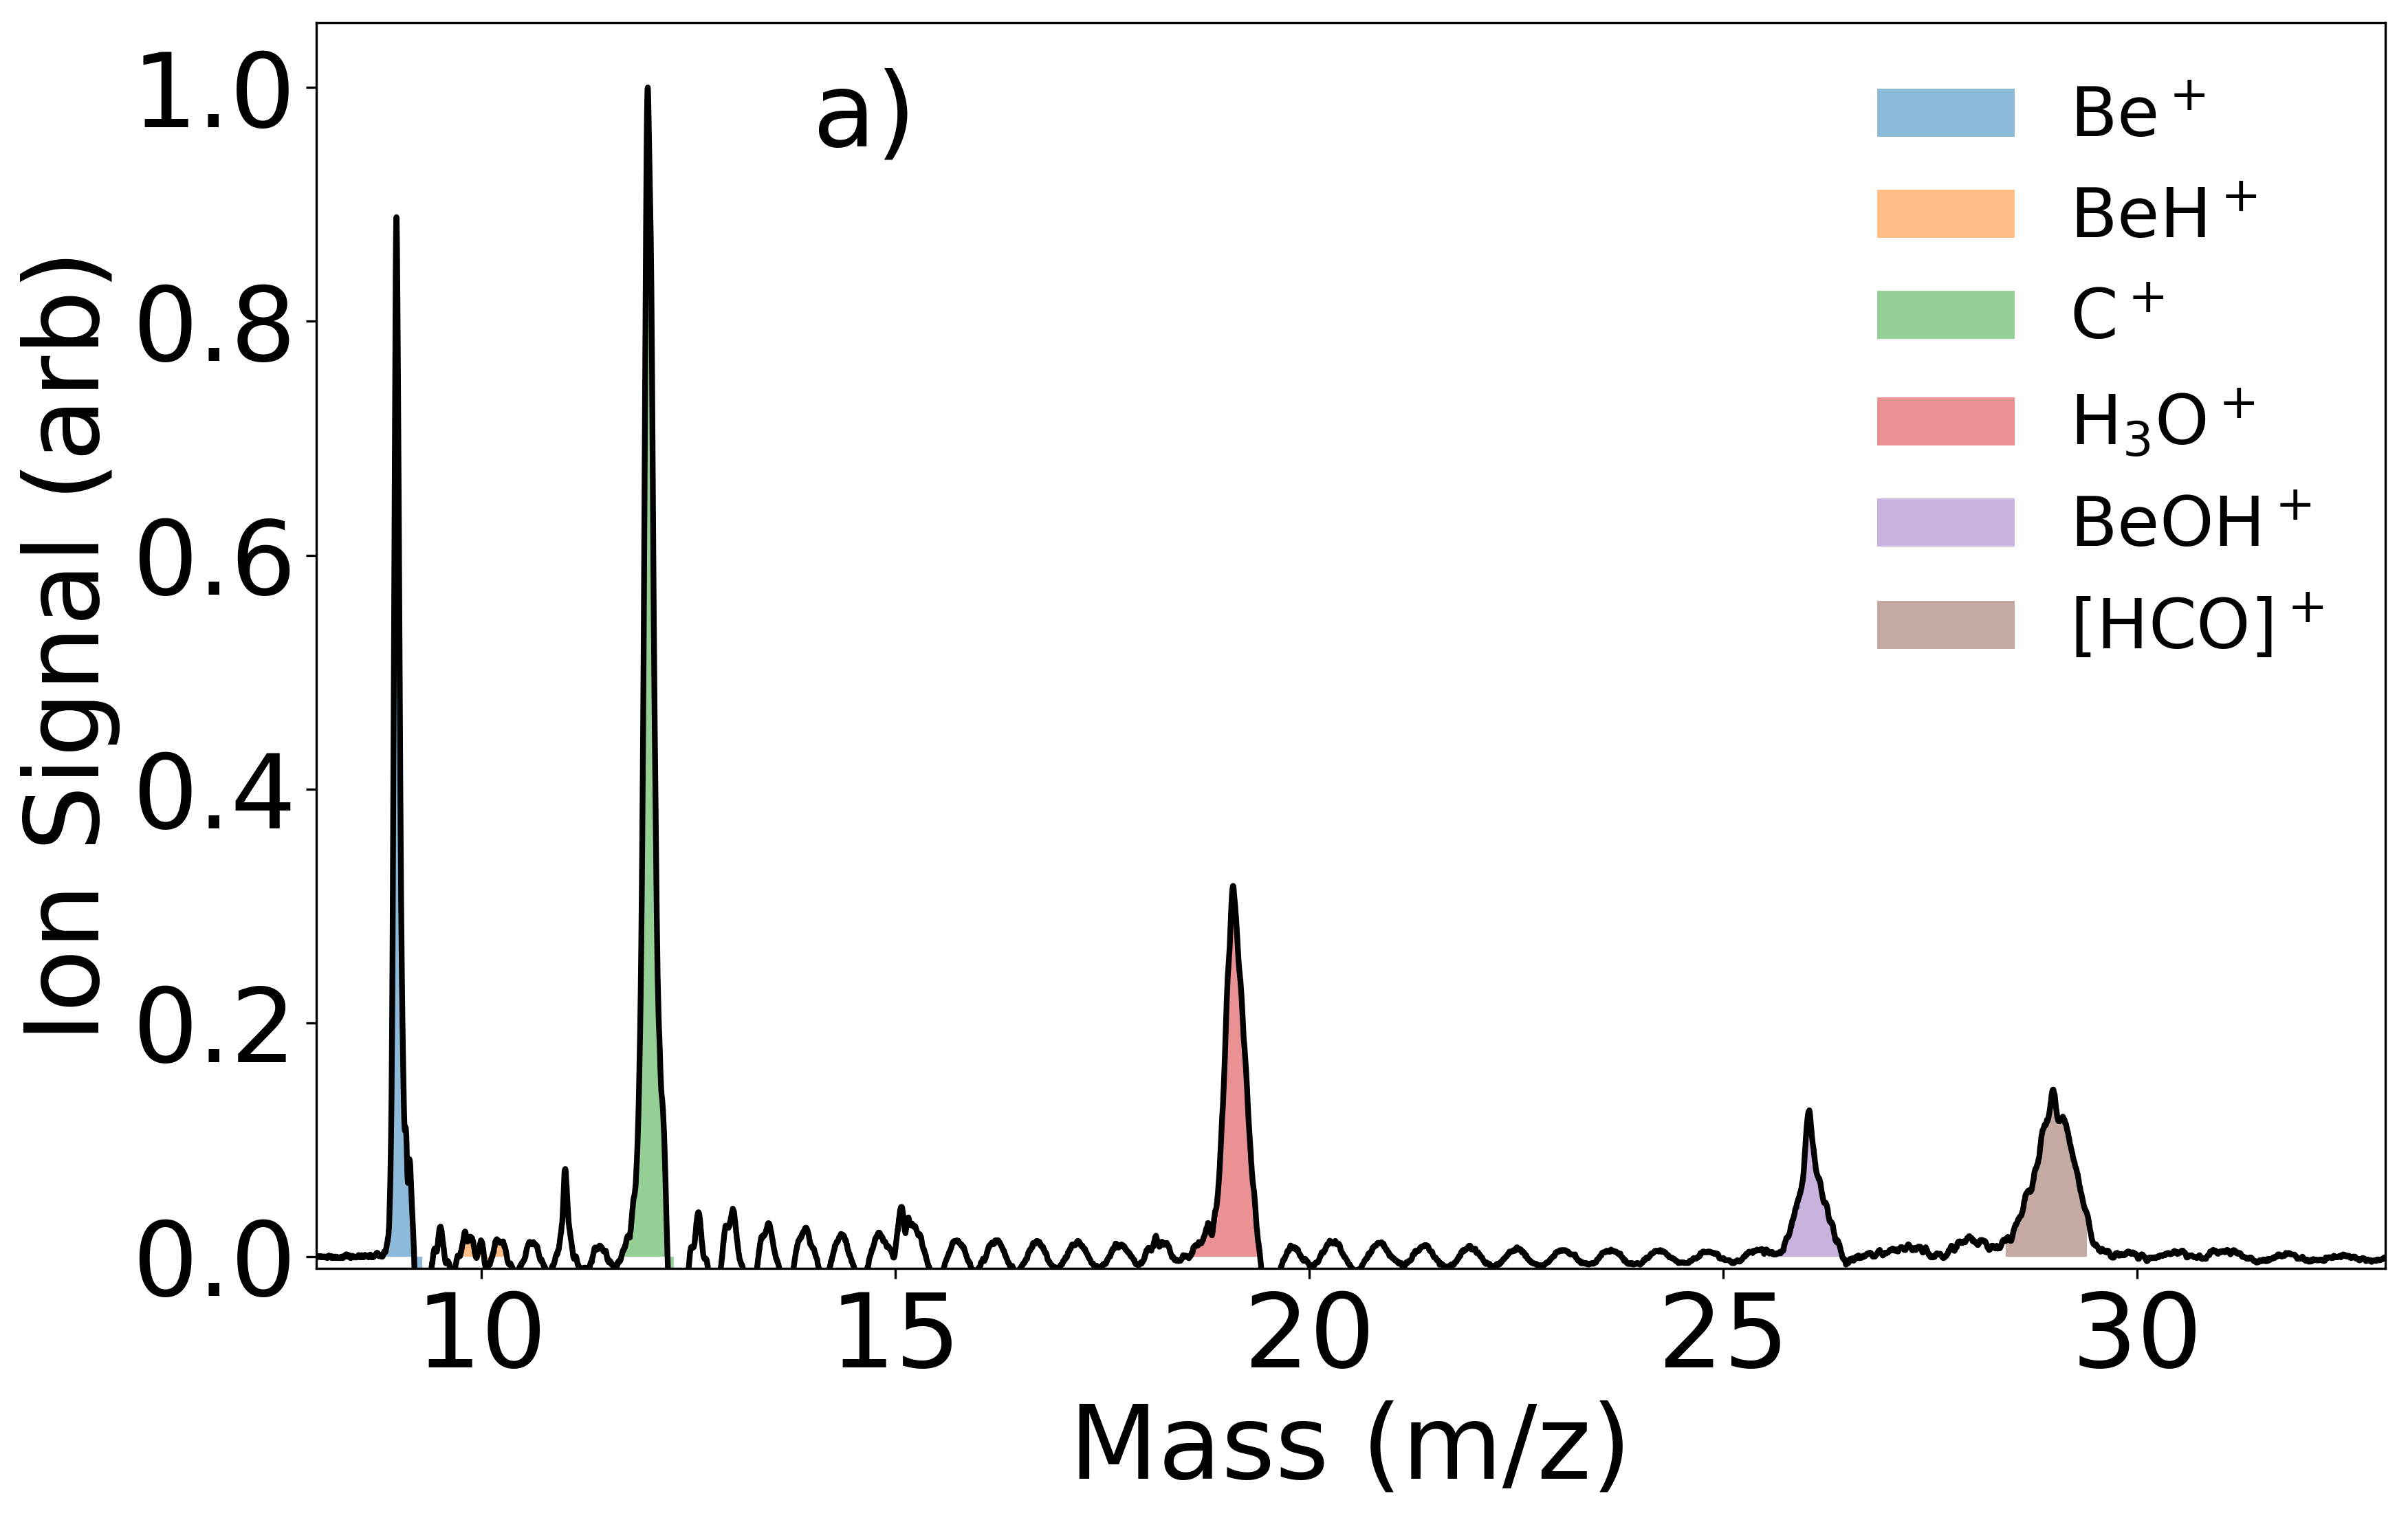
\includegraphics[width=0.5\textwidth]{images/C_H2O_CO_beam_TOF_small.png} &
		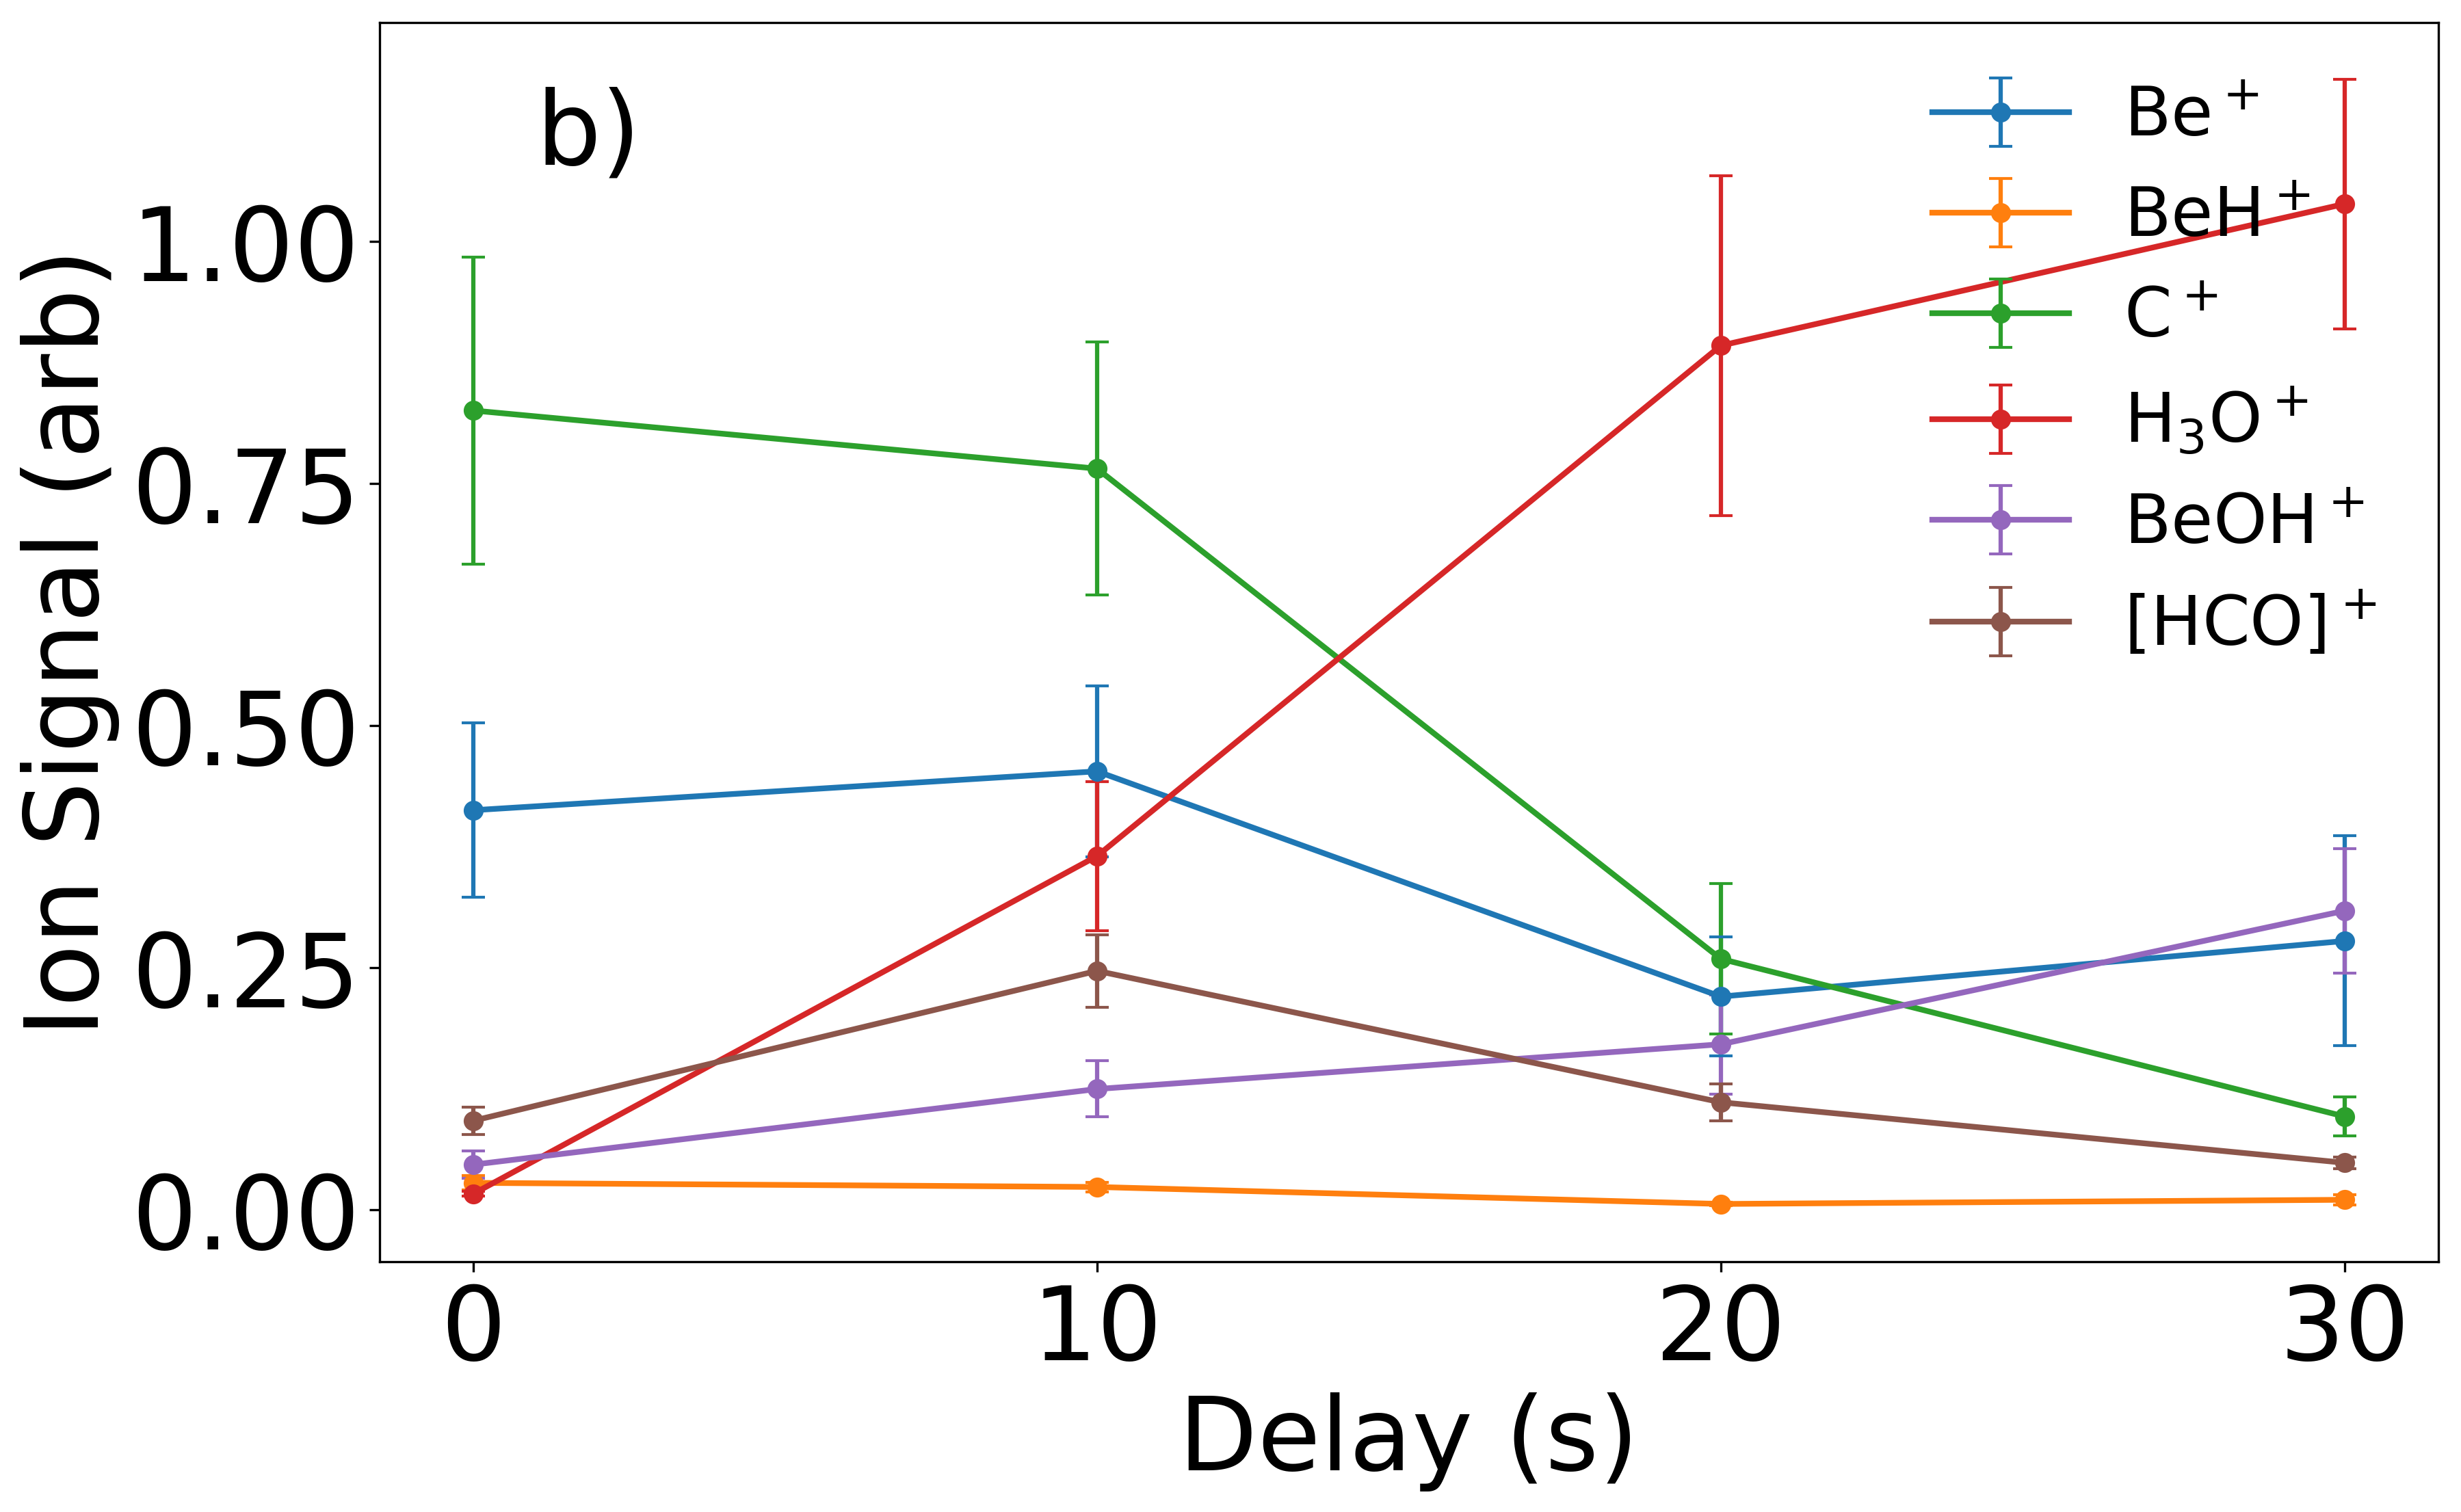
\includegraphics[width=0.5\textwidth]{images/C_H2O_CO_beam_all_traces_small.png}
	\end{tabular}
	}
	\caption{Laser cooled \ce{Be+} with P-state fraction $\approx 20\%$, and \ce{C+} simultaneously react with \ce{H2O} introduced from the CBGB, as well as \ce{CO} introduced from a leak valve. a) A TOF trace of the charged species in the trap after being exposed to \ce{H2O} from the CBGB for 20 s. b) Integrated TOF traces of relevant species at various delay times.}
	\label{fig: Be+CO+H2O+CO all traces}
\end{figure}

By isolating only the integrated peaks for the \ce{Be+ +H2O} network of interest, we may use equation \ref{eq: k Be+H2O(T)} and differential equations in Section \ref{sec: Be+H2O+H2 eqs} to find the density of the \ce{H2O} beam. We set $\rho_{\ce{H2}}=0$ and adjust $k_{\ref{r: Be(P)+H2O->BeOH}}$ for the contribution due to reaction \ref{r: Be(P)+H2O->H2O} in the analysis seen in Figure \ref{fig: Be+C+H2O+CO traces}a). The derived density can then be used to find rate constants for another fitted reaction network, as seen in Figure \ref{fig: Be+C+H2O+CO traces}b), discussed in further detail in Section \ref{sec: [HCO]}.

\begin{figure}[H]
	\centering
	\makebox[\textwidth][c]{
	\begin{tabular}{cc}
		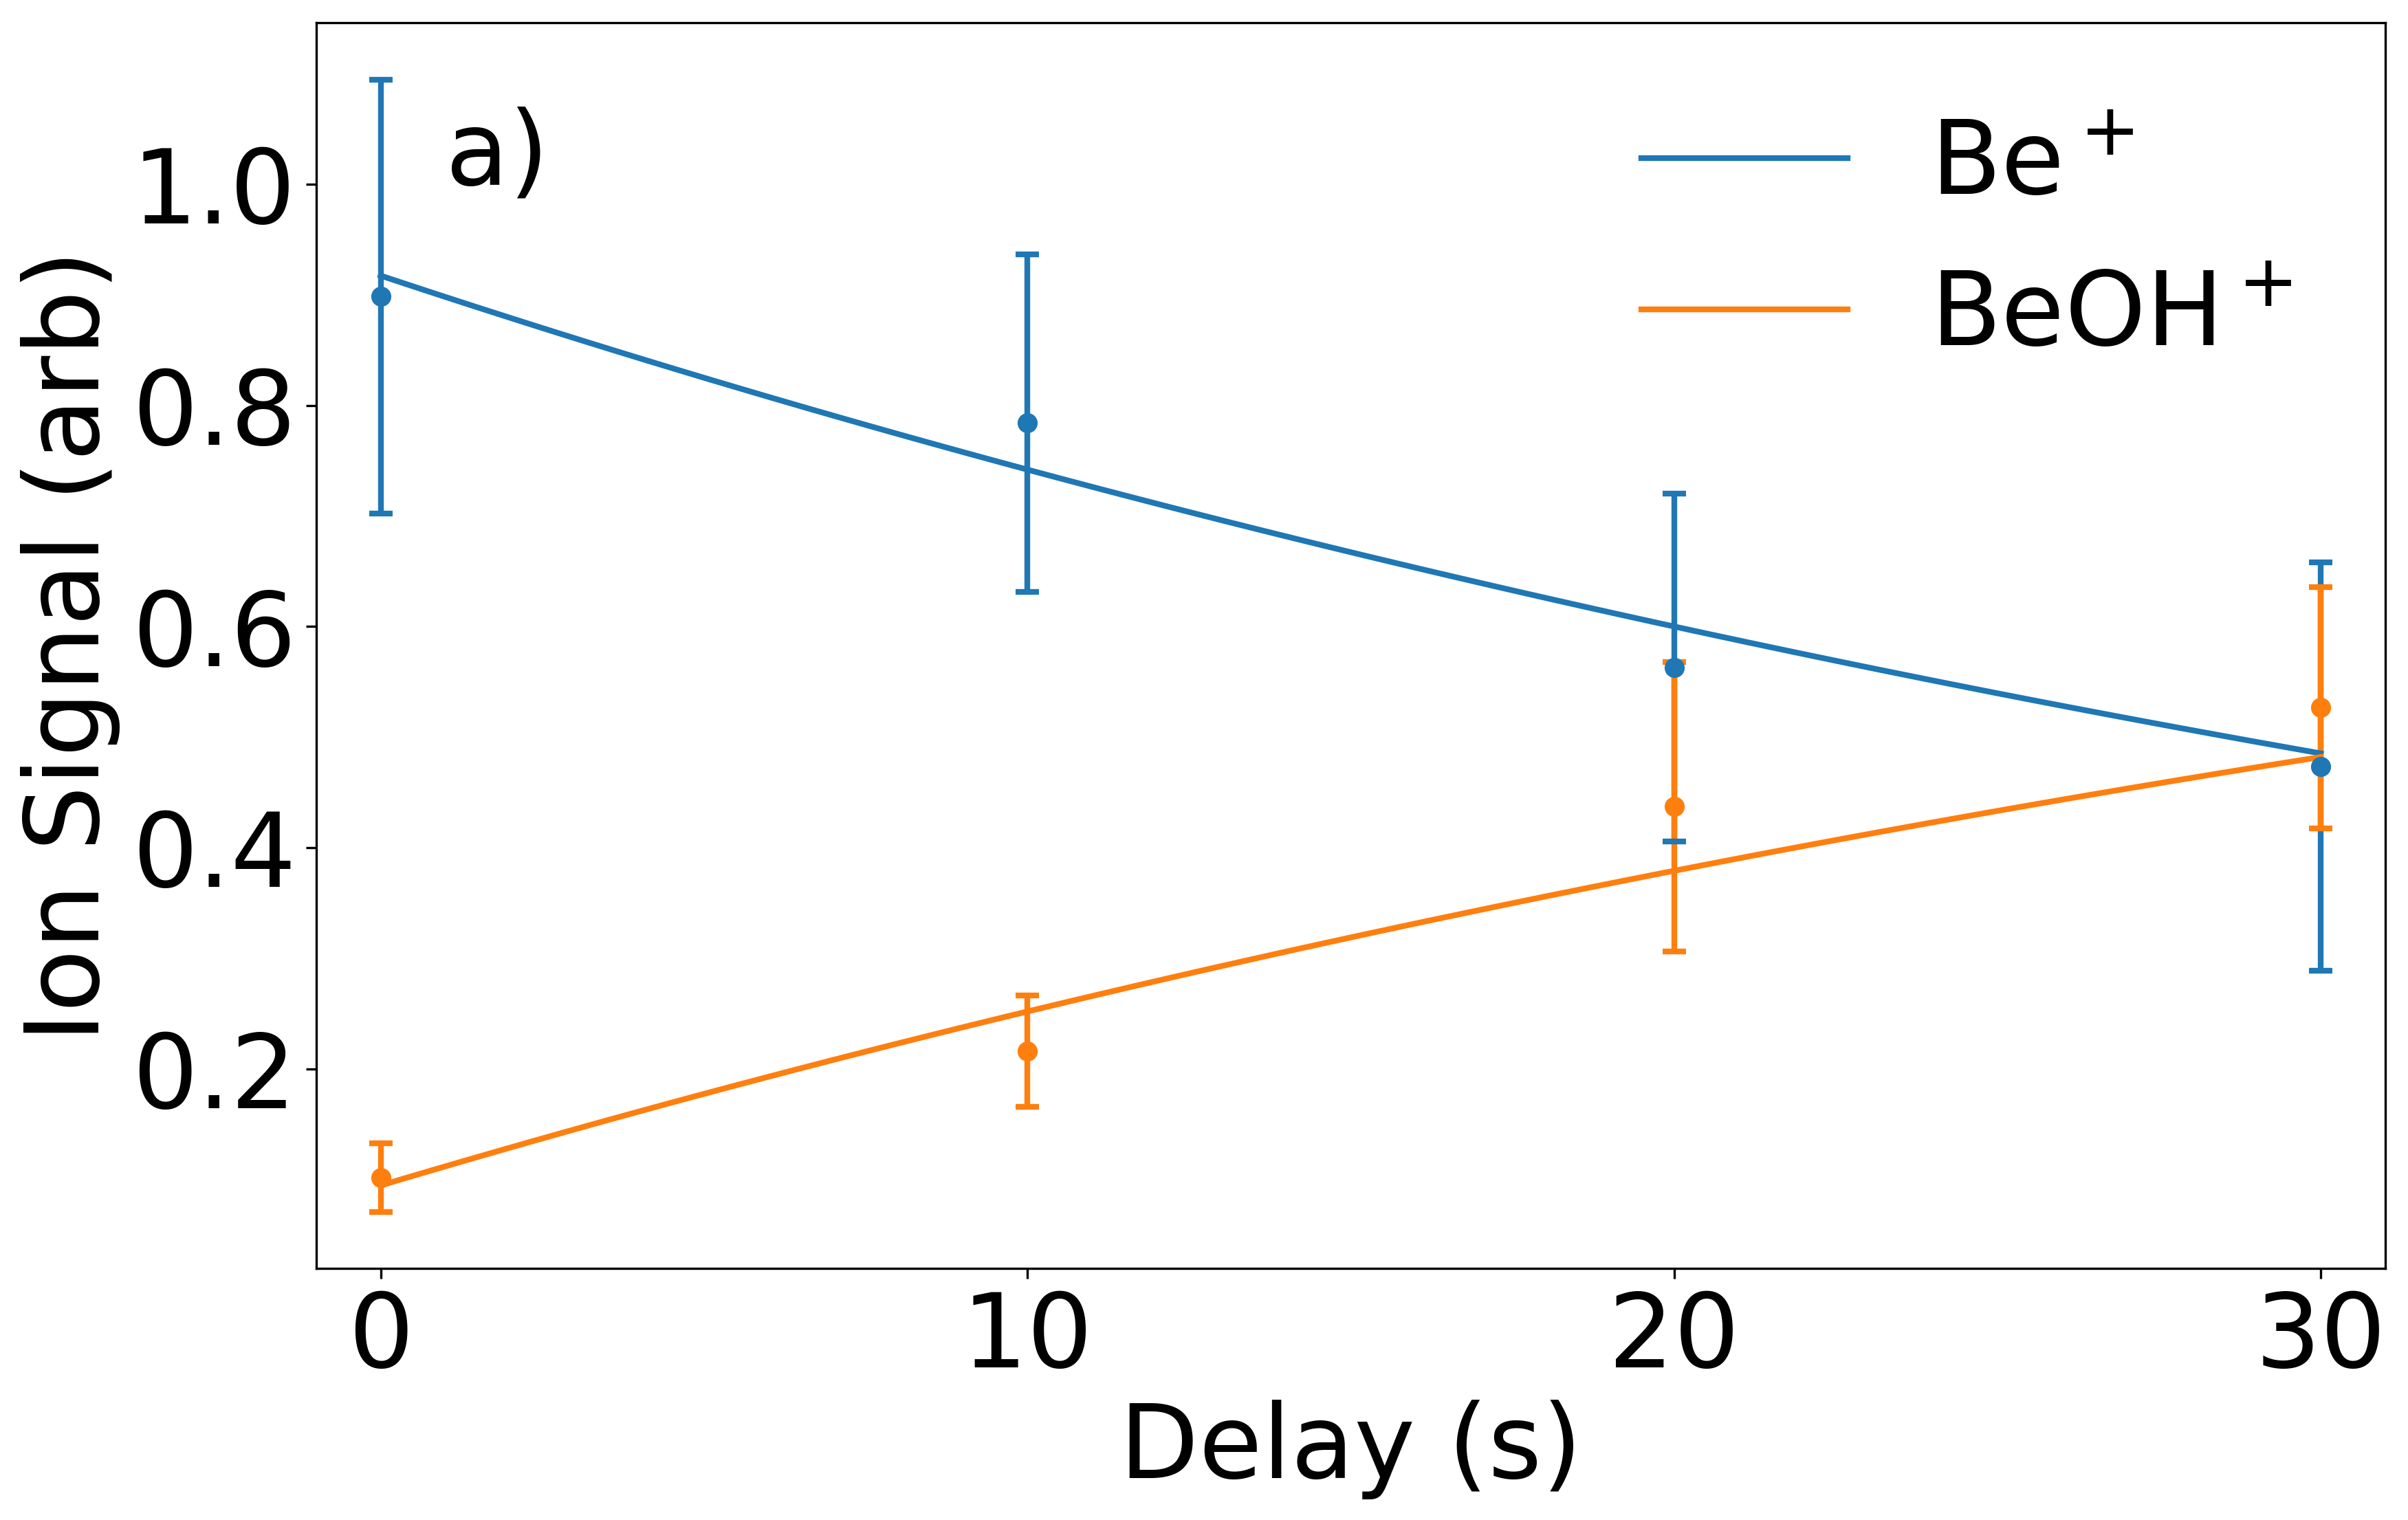
\includegraphics[width=0.5\textwidth]{images/Be_H2O_CO_beam_traces_small.png} &
		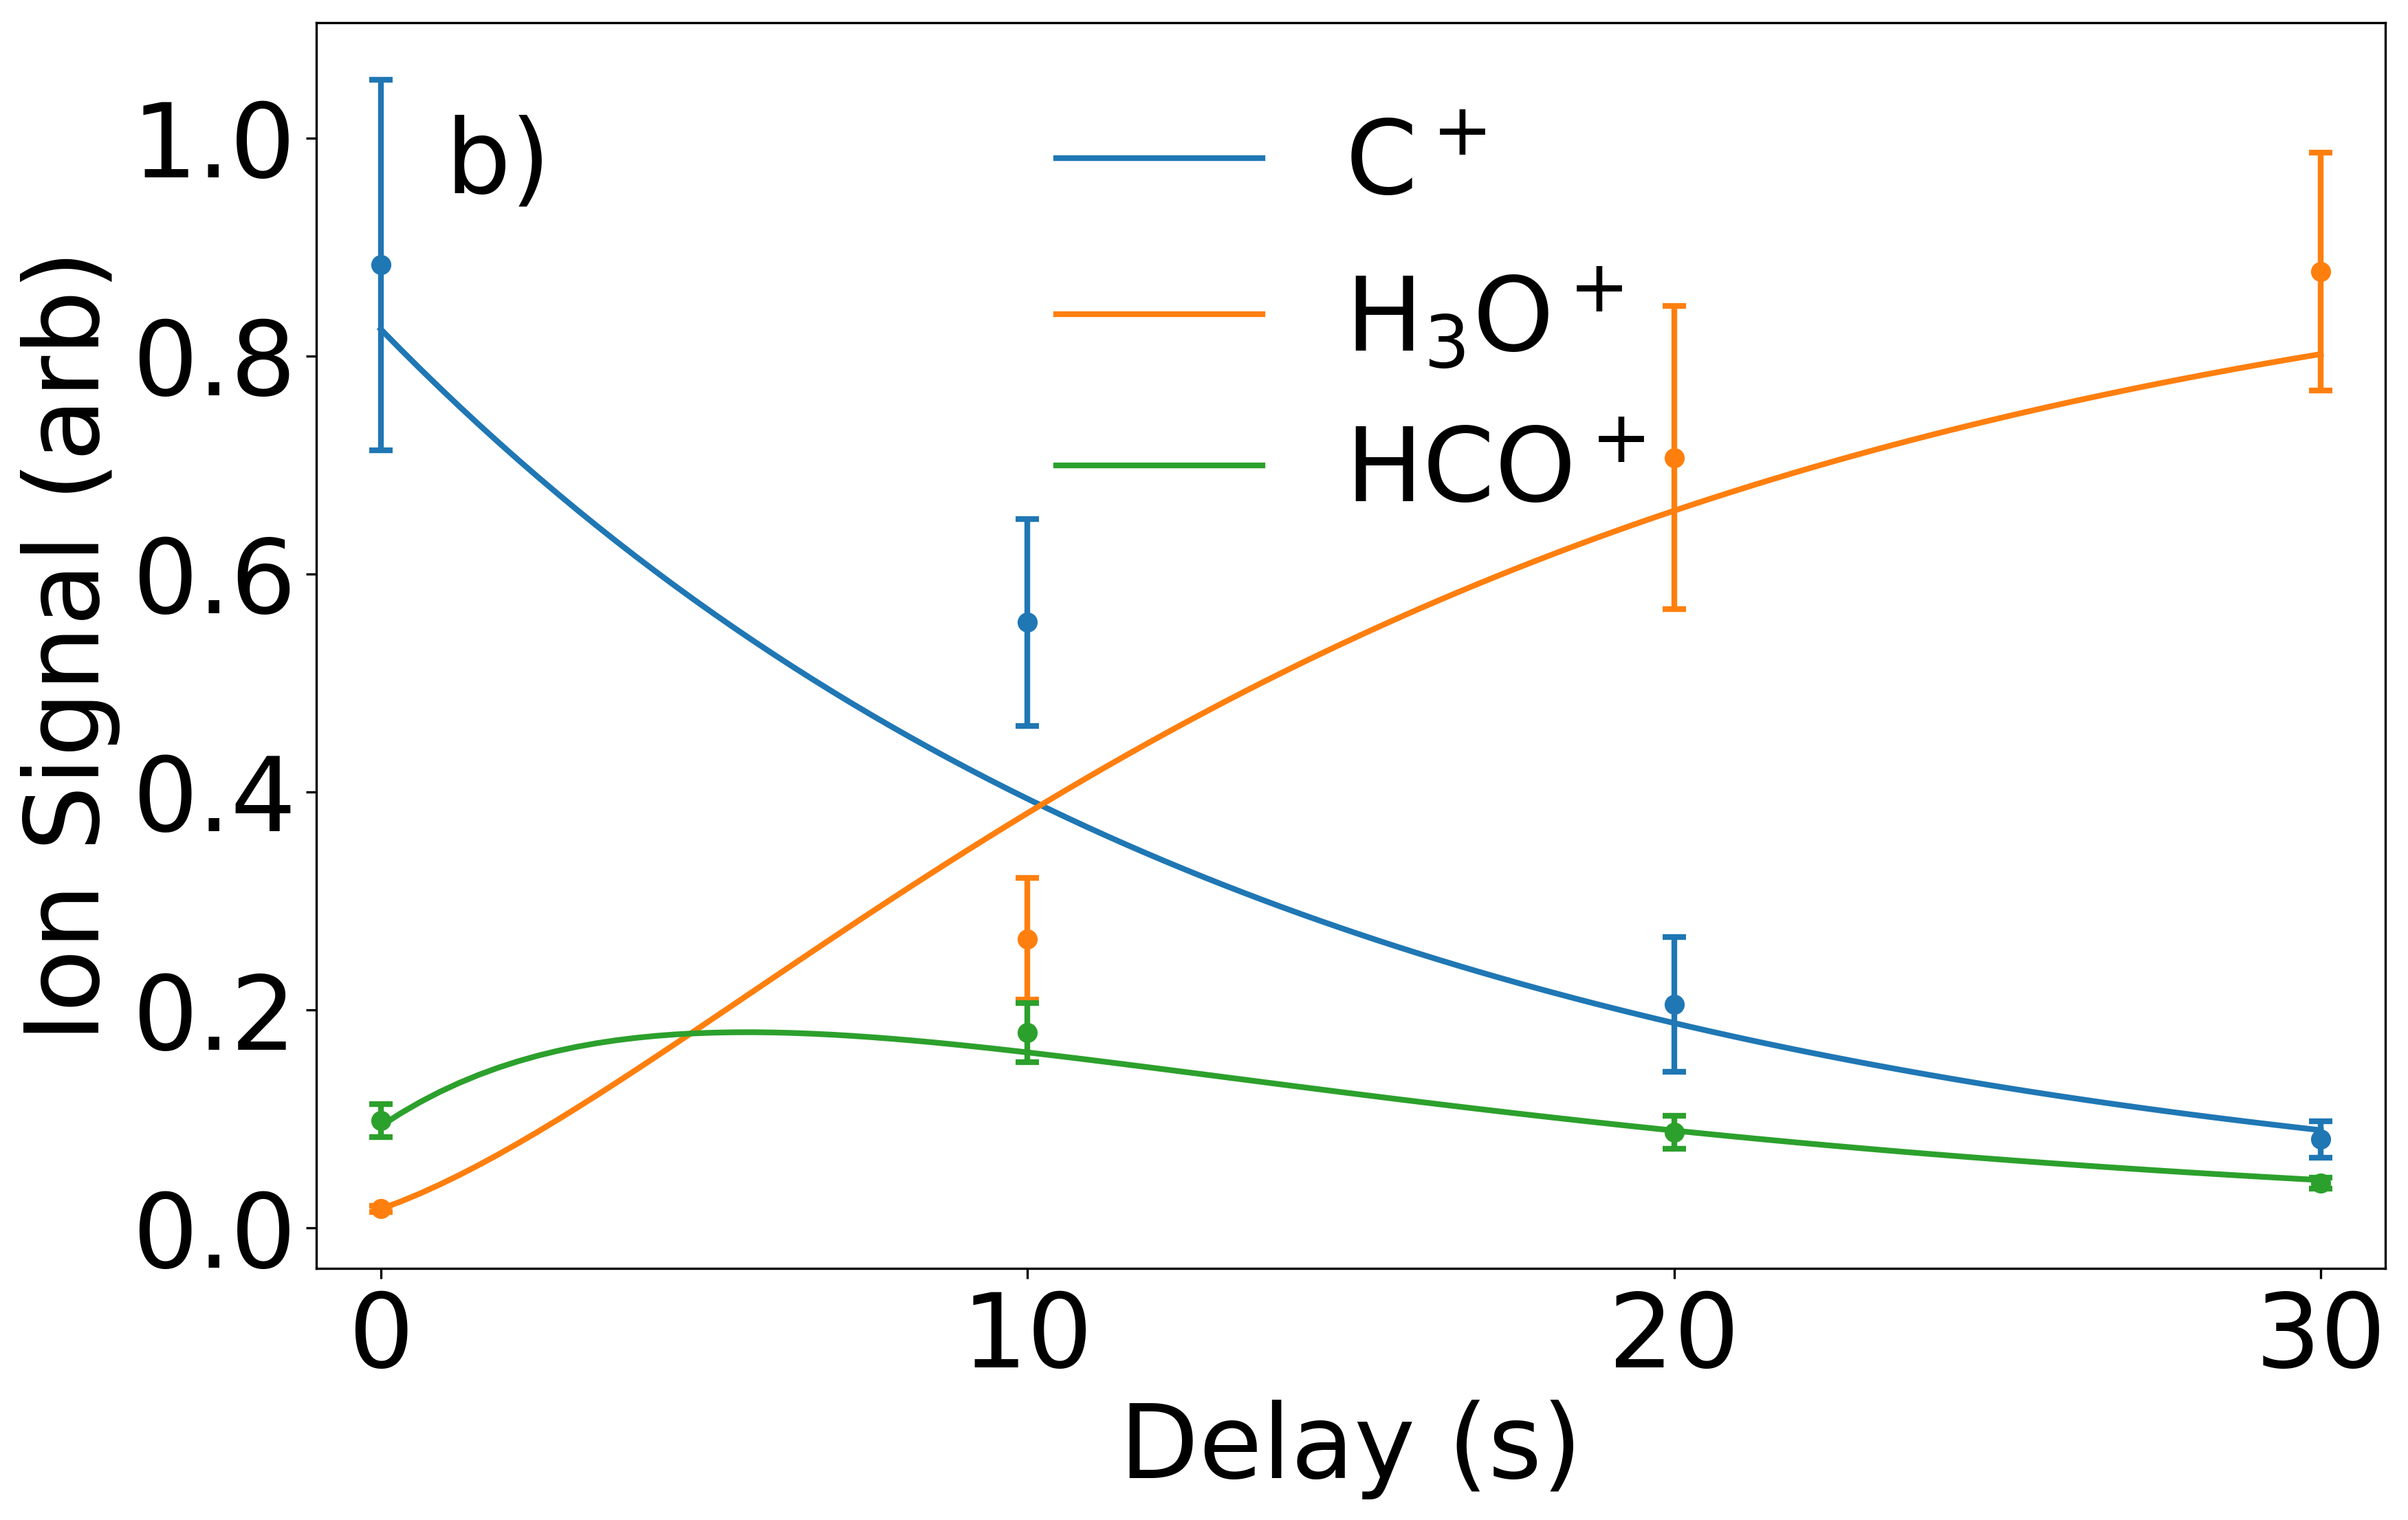
\includegraphics[width=0.5\textwidth]{images/C_H2O_CO_beam_traces_small.png}
	\end{tabular}
	}
	\caption{a) Fitted TOF traces for \ce{Be+ + H2O} reaction network, experimentally derived \ce{H2O} beam density is found to be $\rho_{\ce{H2O}}=(5.4 \pm 0.6) \times 10^6$ 1/cc. b) Isolated and fitted \ce{C+ + H2O} reaction network.}
	\label{fig: Be+C+H2O+CO traces}
\end{figure}

The isolation of reaction networks does not simply reduce the complexity of the shared fitting functions, it is a necessary process. The ablation loading process does not produce the same amount of ions from shot-to-shot, in particular, when considering dual-species loading of \ce{Be+} and \ce{C+}, the ratios will invariably change. The normalization of individual reaction networks is discussed in further detail in Section \ref{sec: dual loading}.